% Motivation frame
\begin{frame}
    \frametitle{Electromagnetic (EM) Applications}
    \begin{figure}
        \centering
        \begin{subfigure}[b]{0.4\textwidth}
            \centering
            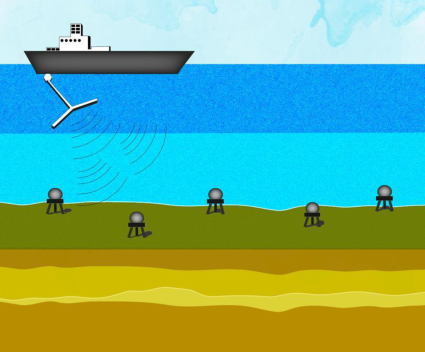
\includegraphics[width=\textwidth]{Diapos/Intro/Figures/csem}
            \caption{CSEM (artificial source)}
        \end{subfigure}
        \hfill
        \begin{subfigure}[b]{0.4\textwidth}
            \centering
            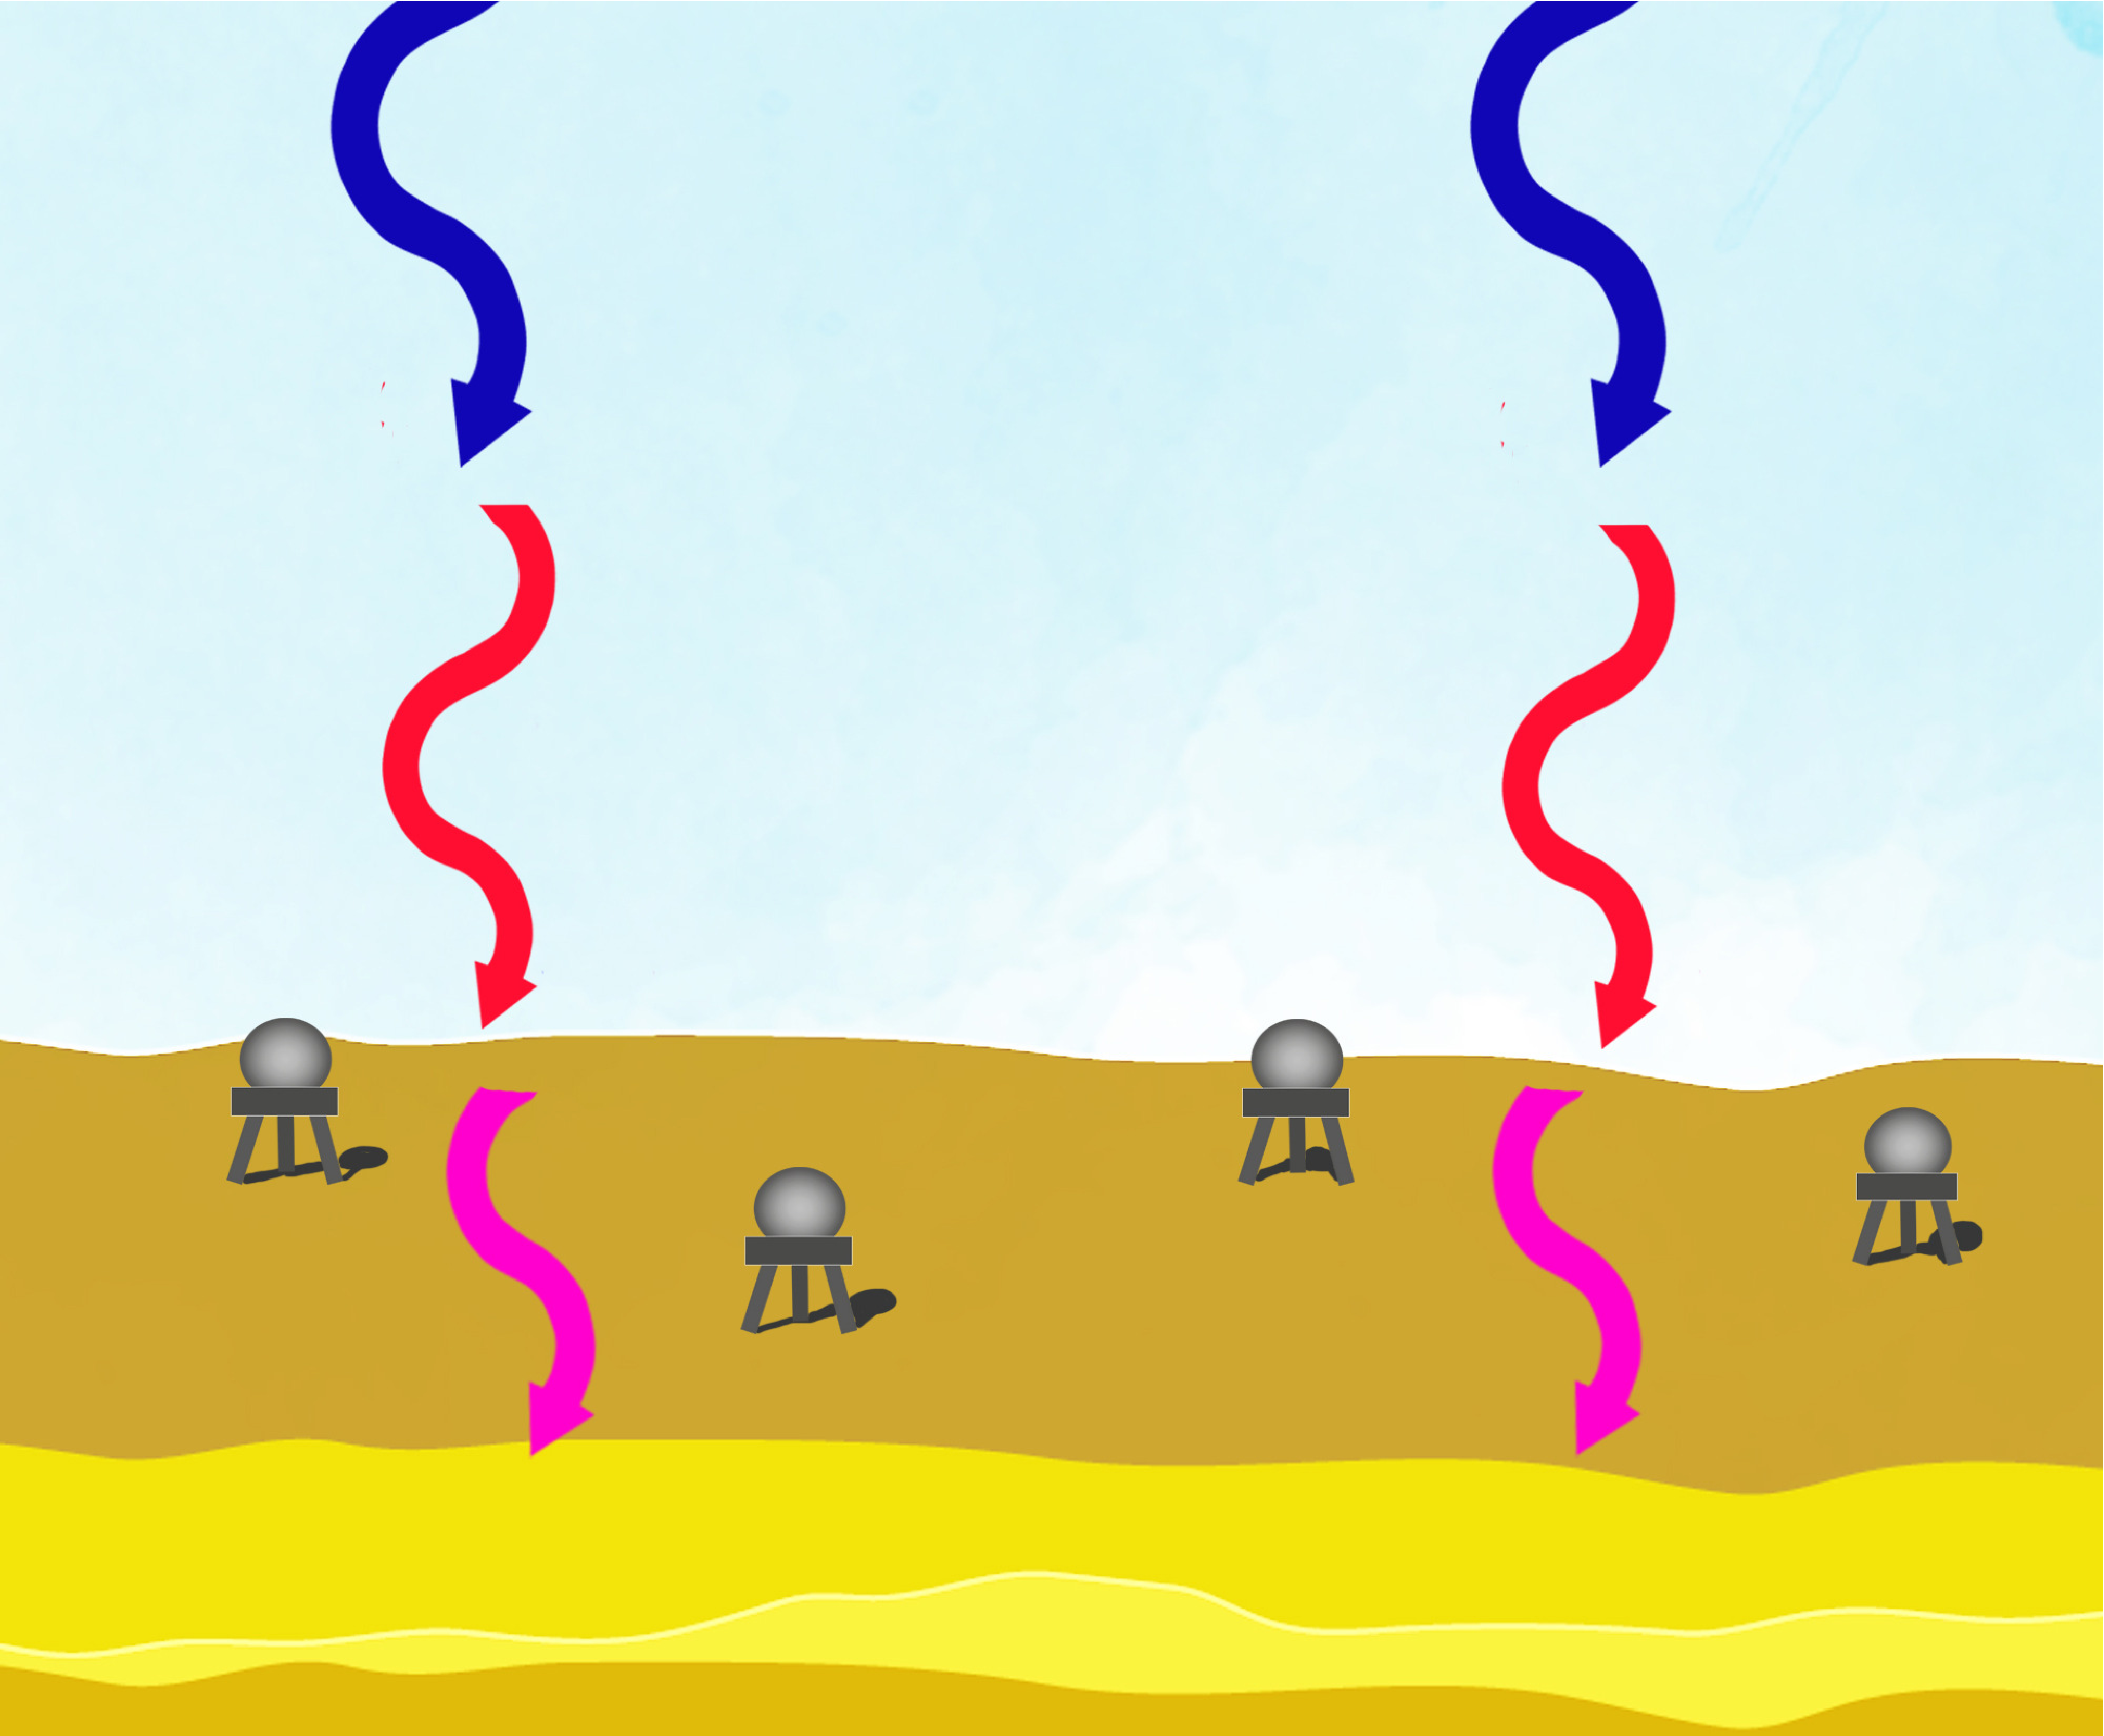
\includegraphics[width=\textwidth]{Diapos/Intro/Figures/magneto}
            \caption{MT (natural source)}
        \end{subfigure}
    \end{figure}
    \vfill
    \begin{block}{Objective}
        \centering
        \textbf{\textcolor{red}{Objective}}: To obtain the \textbf{conductivity/resistivity} distribution \\ of the Earth's subsurface.
    \end{block}
\note[Deep Learning inversion has shown promising results in solving CSEM and MT problems, but it requires large databases for training.]

\end{frame}